\documentclass[tikz,border=8pt]{standalone}
\usepackage{amsmath,amssymb}
\usetikzlibrary{matrix,positioning}
\begin{document}
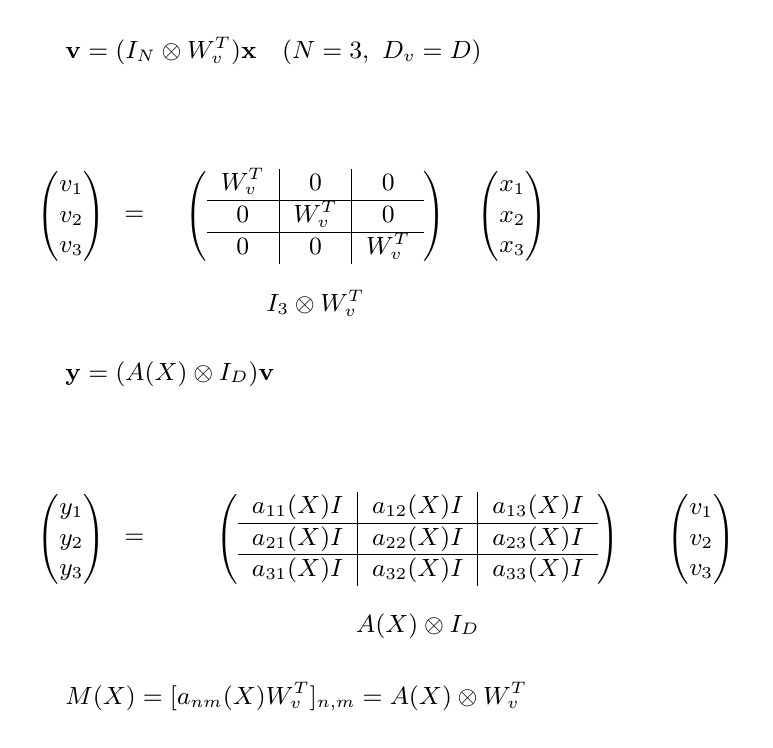
\begin{tikzpicture}[font=\small]
\node[anchor=west] at (0,2.1) {$\mathbf v=(I_N\otimes W_v^T)\mathbf x\quad(N=3,\ D_v=D)$};
\node at (0.2,0) {$\begin{pmatrix}v_1\\v_2\\v_3\end{pmatrix}$};
\node at (1.0,0) {$=$};
\node at (3.3,0) {$\left(\begin{array}{c|c|c}
W_v^T&0&0\\\hline
0&W_v^T&0\\\hline
0&0&W_v^T
\end{array}\right)$};
\node at (5.8,0) {$\begin{pmatrix}x_1\\x_2\\x_3\end{pmatrix}$};
\node at (3.3,-1.1) {$I_3\otimes W_v^T$};
\node[anchor=west] at (0,-2.0) {$\mathbf y=(A(X)\otimes I_D)\mathbf v$};
\node at (0.2,-4.1) {$\begin{pmatrix}y_1\\y_2\\y_3\end{pmatrix}$};
\node at (1.0,-4.1) {$=$};
\node at (4.6,-4.1) {$\left(\begin{array}{c|c|c}
a_{11}(X)I&a_{12}(X)I&a_{13}(X)I\\\hline
a_{21}(X)I&a_{22}(X)I&a_{23}(X)I\\\hline
a_{31}(X)I&a_{32}(X)I&a_{33}(X)I
\end{array}\right)$};
\node at (8.2,-4.1) {$\begin{pmatrix}v_1\\v_2\\v_3\end{pmatrix}$};
\node at (4.6,-5.2) {$A(X)\otimes I_D$};
\node[anchor=west] at (0,-6.1) {$M(X)=[a_{nm}(X)W_v^T]_{n,m}=A(X)\otimes W_v^T$};
\end{tikzpicture}
\end{document}
